\documentclass[aspectratio=169, 12pt]{beamer}
 
\usepackage[utf8]{inputenc}
\usepackage{natbib, url}
\usepackage{enumerate, amsmath, amssymb, amsthm}
\usepackage{ragged2e} % make it justified
\justifying

% \usepackage{enumitem}
% \setlist{itemsep = 0pt, topsep = 1pt, leftmargin = 0.6mm}

\usepackage{hyperref}
\hypersetup{colorlinks, citecolor=blue, urlcolor=blue}
\usepackage{booktabs}
\usepackage{graphicx}


%\mode<presentation>{}
%\usepackage{beamerthemesplit} 

\setbeamertemplate{footline}[frame number]
%\setbeamertemplate{headline}{}
 
% slide 1
%Information to be included in the title page: % cohen was a prominent statistican and psychologist at NYU 
\title{Review of Jacob Cohen's The Earth is Round $(p < .05)$}

\author{Will Quinlan}
 
 
\begin{document}
 
\frame{\titlepage}

 % slide 3
\begin{frame}{An Introduction to Cohen's Paper}
  \begin{itemize}
  \item Scientific advancement has been hindered by null hypothesis testing (NHST)
  \item Researchers often misinterpret p-values restulting in mistakes in what can be concluded
  \item Critique the "ritualization" of NHST 
  \item Focus on real-world relevance
  \item Argues for better scientific practices
  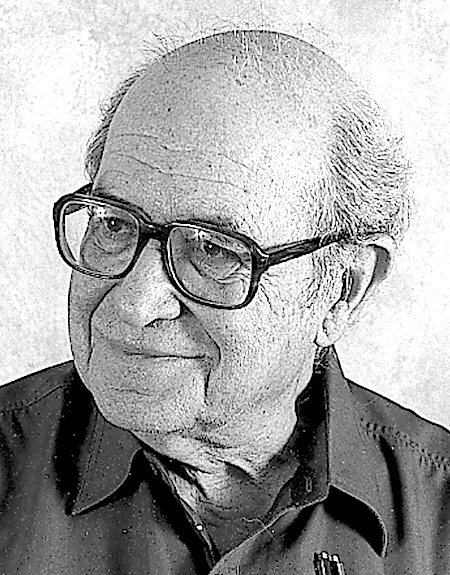
\includegraphics[width=0.15\textwidth]{./images/JacobCohen.png}
  \end{itemize}
\end{frame}

% slide 3
\begin{frame}{On Null Hypothesis Significance Testing}
  \begin{itemize}
  \item Definition: Method of statistical inference by which an experimental factor is tested against a hypothesis of no effect or no relationship based on a given observation
	\begin{itemize}
	\item In other words: Null vs Alternate
	\end{itemize}
  \item p-values determine the signifiance threshold
  \item NHST is dominates science
  \end{itemize}
\end{frame}

%Slide 4
\begin{frame}{A Ritualization of Reasoning $(p < .05)$}
  \begin{itemize}
  \item Cohen argues against the rigid reliance on p-values
  \item 133 registrants through Clubear, our partner in China, thank
    Prof. Hansheng Wang, Peking University
  \item Schizophrenic
    \begin{tabular}{ccccc}
      \toprule
     Result &   Normal & Schiz & Total \\
      \midrule
      Negative Test (Normal)  &  949     &   1           &  950        \\
      Positive Test (Schiz)  &  30      &    20          &  50        \\
      Total    &  979      & 21          & 1,000         \\
      \bottomrule
    \end{tabular}
  \end{itemize}
\end{frame}

% Slide 5
\begin{frame}{Misinterpretation of p-values}
\begin{itemize} %[parsep=0pt, leftmargin=4mm, topsep=0pt, itemsep=0pt]
\item
Alison Lukan, Seattle Kraken Contributor and TV Analyst for Root
 Sports
 \item
 Brian Macdonald, Lecturer, Department of Statistics and Data
 Science, Yale University
\item
Gregory J. Matthews, Associate Professor, Statistics, Loyola
University Chicago
\item  
Lauren (Poe) Parolin, Sports Analytics Developer, ESPN
\item
 Jun Yan (Chair), Professor of Statistics, University of Connecticut
 \end{itemize}
\end{frame}

%Slide 6
\begin{frame}{The Illusion of Proof}
  \begin{itemize}
  \item Virtual participants: put questions into the Q/A window in WebEx
  \item In-person participants: walk to a microphone and wait to be called upon
    before asking your question
  \item Lunch on your own (Student Union food court right next door)x
  \item Coffee/cookies available during the poster session (11:30--13:30)
  \item Training workshops:
    \begin{itemize}
    \item Each workshop has its own (webex meeting) room
    \item Virtual participants please mute yourself in each session.
    \end{itemize}
  \end{itemize}
\end{frame}

%Slide 7
\begin{frame}{The Illusion of Proof}
  \begin{itemize}
  \item Virtual participants: put questions into the Q/A window in WebEx
  \item In-person participants: walk to a microphone and wait to be called upon
    before asking your question
  \item Lunch on your own (Student Union food court right next door)x
  \item Coffee/cookies available during the poster session (11:30--13:30)
  \item Training workshops:
    \begin{itemize}
    \item Each workshop has its own (webex meeting) room
    \item Virtual participants please mute yourself in each session.
    \end{itemize}
  \end{itemize}
\end{frame}

%Slide 8
\begin{frame}{The Illusion of Proof}
  \begin{itemize}
  \item Virtual participants: put questions into the Q/A window in WebEx
  \item In-person participants: walk to a microphone and wait to be called upon
    before asking your question
  \item Lunch on your own (Student Union food court right next door)x
  \item Coffee/cookies available during the poster session (11:30--13:30)
  \item Training workshops:
    \begin{itemize}
    \item Each workshop has its own (webex meeting) room
    \item Virtual participants please mute yourself in each session.
    \end{itemize}
  \end{itemize}
\end{frame}

%Slide 8
\begin{frame}{The Illusion of Proof}
  \begin{itemize}
  \item Virtual participants: put questions into the Q/A window in WebEx
  \item In-person participants: walk to a microphone and wait to be called upon
    before asking your question
  \item Lunch on your own (Student Union food court right next door)x
  \item Coffee/cookies available during the poster session (11:30--13:30)
  \item Training workshops:
    \begin{itemize}
    \item Each workshop has its own (webex meeting) room
    \item Virtual participants please mute yourself in each session.
    \end{itemize}
  \end{itemize}
\end{frame}

%Slide 10
\begin{frame}{The Illusion of Proof}
  \begin{itemize}
  \item Virtual participants: put questions into the Q/A window in WebEx
  \item In-person participants: walk to a microphone and wait to be called upon
    before asking your question
  \item Lunch on your own (Student Union food court right next door)x
  \item Coffee/cookies available during the poster session (11:30--13:30)
  \item Training workshops:
    \begin{itemize}
    \item Each workshop has its own (webex meeting) room
    \item Virtual participants please mute yourself in each session.
    \end{itemize}
  \end{itemize}
\end{frame}

%Slide 11
\begin{frame}{The Illusion of Proof}
  \begin{itemize}
  \item Virtual participants: put questions into the Q/A window in WebEx
  \item In-person participants: walk to a microphone and wait to be called upon
    before asking your question
  \item Lunch on your own (Student Union food court right next door)x
  \item Coffee/cookies available during the poster session (11:30--13:30)
  \item Training workshops:
    \begin{itemize}
    \item Each workshop has its own (webex meeting) room
    \item Virtual participants please mute yourself in each session.
    \end{itemize}
  \end{itemize}
\end{frame}

%Slide 12
\begin{frame}{The Illusion of Proof}
  \begin{itemize}
  \item Virtual participants: put questions into the Q/A window in WebEx
  \item In-person participants: walk to a microphone and wait to be called upon
    before asking your question
  \item Lunch on your own (Student Union food court right next door)x
  \item Coffee/cookies available during the poster session (11:30--13:30)
  \item Training workshops:
    \begin{itemize}
    \item Each workshop has its own (webex meeting) room
    \item Virtual participants please mute yourself in each session.
    \end{itemize}
  \end{itemize}
\end{frame}

%Slide 13
\begin{frame}{The Illusion of Proof}
  \begin{itemize}
  \item Virtual participants: put questions into the Q/A window in WebEx
  \item In-person participants: walk to a microphone and wait to be called upon
    before asking your question
  \item Lunch on your own (Student Union food court right next door)x
  \item Coffee/cookies available during the poster session (11:30--13:30)
  \item Training workshops:
    \begin{itemize}
    \item Each workshop has its own (webex meeting) room
    \item Virtual participants please mute yourself in each session.
    \end{itemize}
  \end{itemize}
\end{frame}

%Slide 14
\begin{frame}{The Illusion of Proof}
  \begin{itemize}
  \item Virtual participants: put questions into the Q/A window in WebEx
  \item In-person participants: walk to a microphone and wait to be called upon
    before asking your question
  \item Lunch on your own (Student Union food court right next door)x
  \item Coffee/cookies available during the poster session (11:30--13:30)
  \item Training workshops:
    \begin{itemize}
    \item Each workshop has its own (webex meeting) room
    \item Virtual participants please mute yourself in each session.
    \end{itemize}
  \end{itemize}
\end{frame}

%Slide 15
\begin{frame}{The Illusion of Proof}
  \begin{itemize}
  \item Virtual participants: put questions into the Q/A window in WebEx
  \item In-person participants: walk to a microphone and wait to be called upon
    before asking your question
  \item Lunch on your own (Student Union food court right next door)x
  \item Coffee/cookies available during the poster session (11:30--13:30)
  \item Training workshops:
    \begin{itemize}
    \item Each workshop has its own (webex meeting) room
    \item Virtual participants please mute yourself in each session.
    \end{itemize}
  \end{itemize}
\end{frame}

%Slide 16
\begin{frame}{The Illusion of Proof}
  \begin{itemize}
  \item Virtual participants: put questions into the Q/A window in WebEx
  \item In-person participants: walk to a microphone and wait to be called upon
    before asking your question
  \item Lunch on your own (Student Union food court right next door)x
  \item Coffee/cookies available during the poster session (11:30--13:30)
  \item Training workshops:
    \begin{itemize}
    \item Each workshop has its own (webex meeting) room
    \item Virtual participants please mute yourself in each session.
    \end{itemize}
  \end{itemize}
\end{frame}

%Slide 17
\begin{frame}{The Illusion of Proof}
  \begin{itemize}
  \item Virtual participants: put questions into the Q/A window in WebEx
  \item In-person participants: walk to a microphone and wait to be called upon
    before asking your question
  \item Lunch on your own (Student Union food court right next door)x
  \item Coffee/cookies available during the poster session (11:30--13:30)
  \item Training workshops:
    \begin{itemize}
    \item Each workshop has its own (webex meeting) room
    \item Virtual participants please mute yourself in each session.
    \end{itemize}
  \end{itemize}
\end{frame}

%Slide 18
\begin{frame}{The Illusion of Proof}
  \begin{itemize}
  \item Virtual participants: put questions into the Q/A window in WebEx
  \item In-person participants: walk to a microphone and wait to be called upon
    before asking your question
  \item Lunch on your own (Student Union food court right next door)x
  \item Coffee/cookies available during the poster session (11:30--13:30)
  \item Training workshops:
    \begin{itemize}
    \item Each workshop has its own (webex meeting) room
    \item Virtual participants please mute yourself in each session.
    \end{itemize}
  \end{itemize}
\end{frame}

%Slide 19
\begin{frame}{The Illusion of Proof}
  \begin{itemize}
  \item Virtual participants: put questions into the Q/A window in WebEx
  \item In-person participants: walk to a microphone and wait to be called upon
    before asking your question
  \item Lunch on your own (Student Union food court right next door)x
  \item Coffee/cookies available during the poster session (11:30--13:30)
  \item Training workshops:
    \begin{itemize}
    \item Each workshop has its own (webex meeting) room
    \item Virtual participants please mute yourself in each session.
    \end{itemize}
  \end{itemize}
\end{frame}

%Slide 20
\begin{frame}{The Illusion of Proof}
  \begin{itemize}
  \item Virtual participants: put questions into the Q/A window in WebEx
  \item In-person participants: walk to a microphone and wait to be called upon
    before asking your question
  \item Lunch on your own (Student Union food court right next door)x
  \item Coffee/cookies available during the poster session (11:30--13:30)
  \item Training workshops:
    \begin{itemize}
    \item Each workshop has its own (webex meeting) room
    \item Virtual participants please mute yourself in each session.
    \end{itemize}
  \end{itemize}
\end{frame}
%Slide 21
\begin{frame}{The Illusion of Proof}
  \begin{itemize}
  \item Virtual participants: put questions into the Q/A window in WebEx
  \item In-person participants: walk to a microphone and wait to be called upon
    before asking your question
  \item Lunch on your own (Student Union food court right next door)x
  \item Coffee/cookies available during the poster session (11:30--13:30)
  \item Training workshops:
    \begin{itemize}
    \item Each workshop has its own (webex meeting) room
    \item Virtual participants please mute yourself in each session.
    \end{itemize}
  \end{itemize}
\end{frame}


\end{document}
